%                                                                 aa.dem
% AA vers. 9.1, LaTeX class for Astronomy & Astrophysics
% demonstration file
%                                                       (c) EDP Sciences
%-----------------------------------------------------------------------
%
%\documentclass[referee]{aa} % for a referee version
%\documentclass[onecolumn]{aa} % for a paper on 1 column  
%\documentclass[longauth]{aa} % for the long lists of affiliations 
%\documentclass[letter]{aa} % for the letters 
%\documentclass[bibyear]{aa} % if the references are not structured 
%                              according to the author-year natbib style

%
\documentclass{aa}  
\renewcommand{\arraystretch}{1.4}
\graphicspath{ {./imgs/} }

%
\usepackage{graphicx}
\usepackage{lscape}
%%%%%%%%%%%%%%%%%%%%%%%%%%%%%%%%%%%%%%%%
\usepackage{txfonts}
%%%%%%%%%%%%%%%%%%%%%%%%%%%%%%%%%%%%%%%%
%\usepackage[options]{hyperref}
% To add links in your PDF file, use the package "hyperref"
% with options according to your LaTeX or PDFLaTeX drivers.
%
\begin{document} 


   \title{Chemistry Study on Hot Corino Serpen South CARMA-7}



   \author{Haotian Liu (under supervision of Dr. Adele L. Plunkett)}

   \institute{University of Virginia,
              \email{hl7gr@virginia.edu}}




% \abstract{}{}{}{}{} 
% 5 {} token are mandatory
 
  \abstract
  % context heading (optional)
  % {} leave it empty if necessary  
   {To study the interesting chemistry of a newly found hot corino CARMA-7 in Serpen South region}
  % aims heading (mandatory)
   {Chemical line identification and source motion analysis}
  % methods heading (mandatory)
   {CASA ADMIT + other spectral processing tools}
  % results heading (mandatory)
   {See line identification and conclusion}
  % conclusions heading (optional), leave it empty if necessary 
   {}

   \keywords{Hot corino, Astrochemistry, Scientific computing}

   \maketitle
%
%-------------------------------------------------------------------

\section{Introduction}

    This thesis contains spectral line analysis of 6 spectral windows of ALMA observation on source Serpen South CARMA-7.

%--------------------------------------------------------------------
\section{Observation}
   ALMA observation was conducted with 6 spectral windows.
   \begin{figure*}
    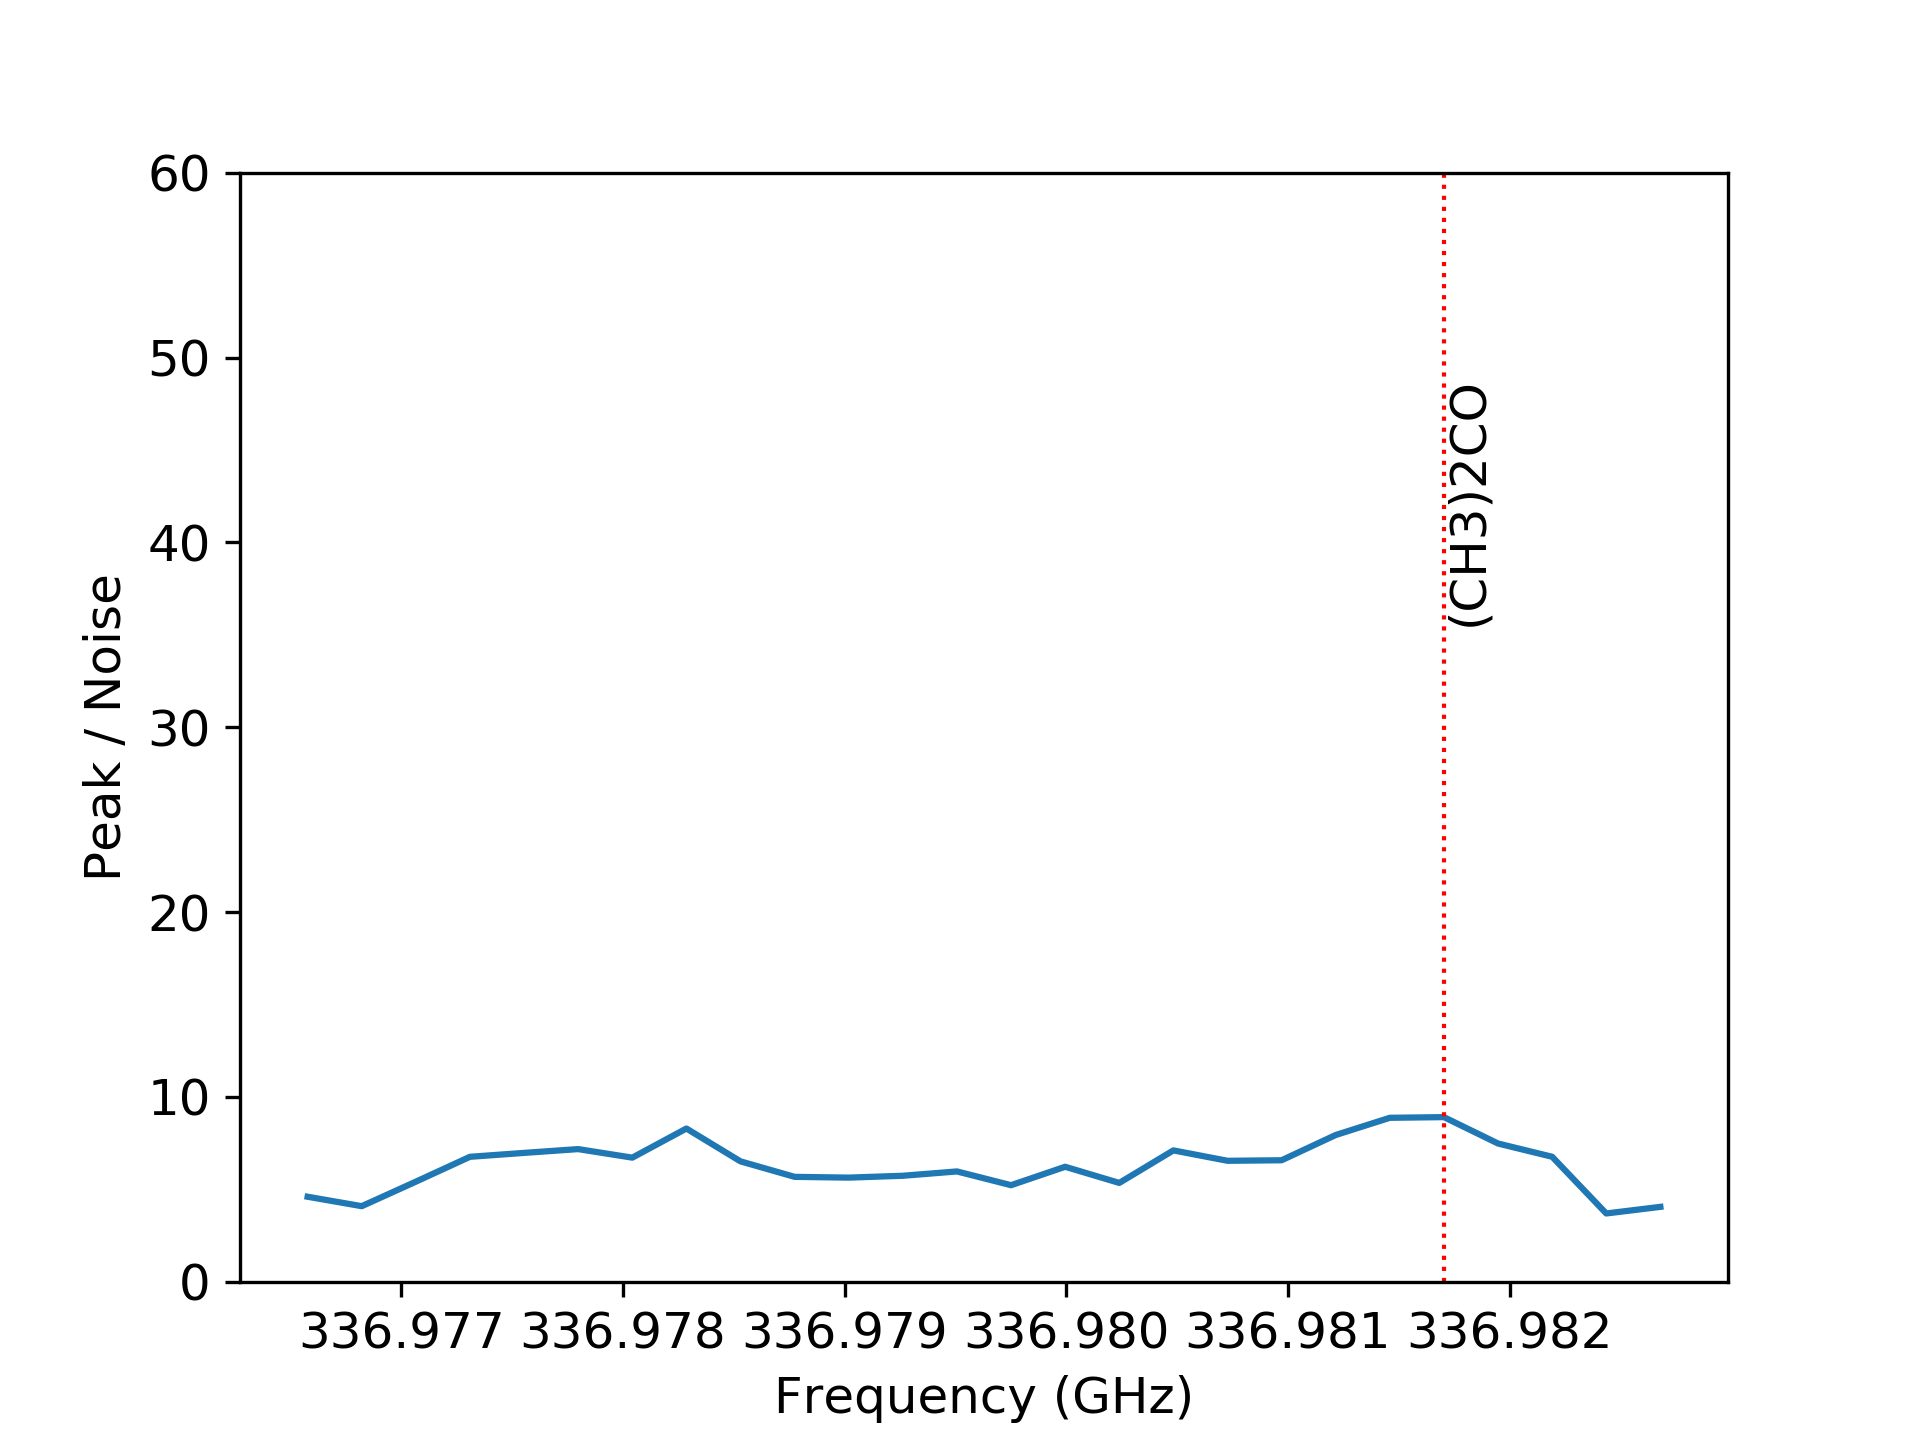
\includegraphics[width=0.33\textwidth]{spw0_(CH3)2CO}
    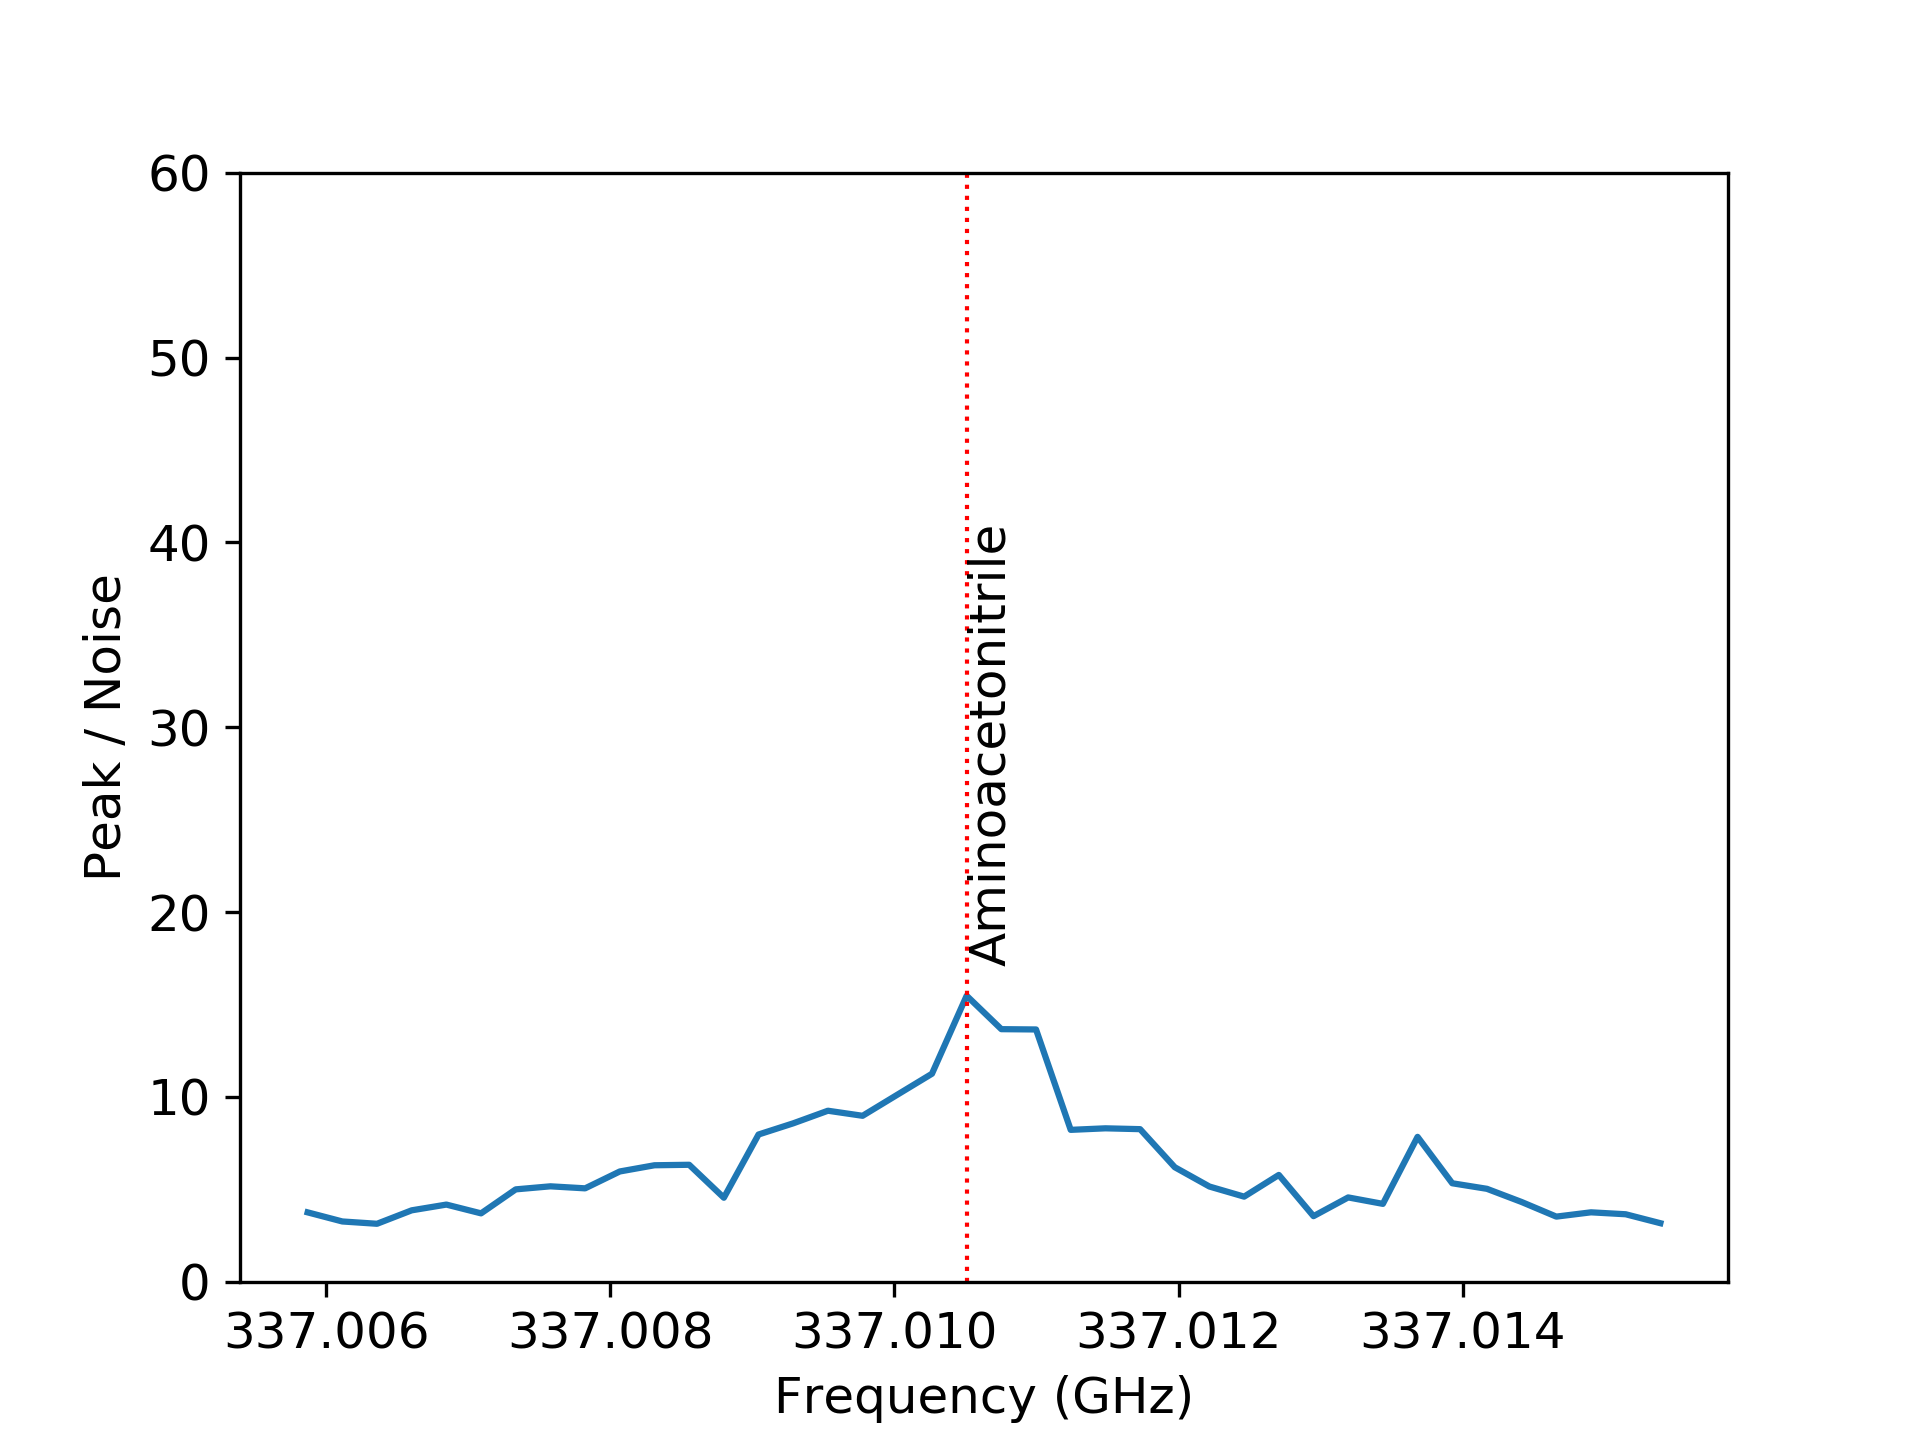
\includegraphics[width=0.33\textwidth]{spw0_H2NCH2CN}
    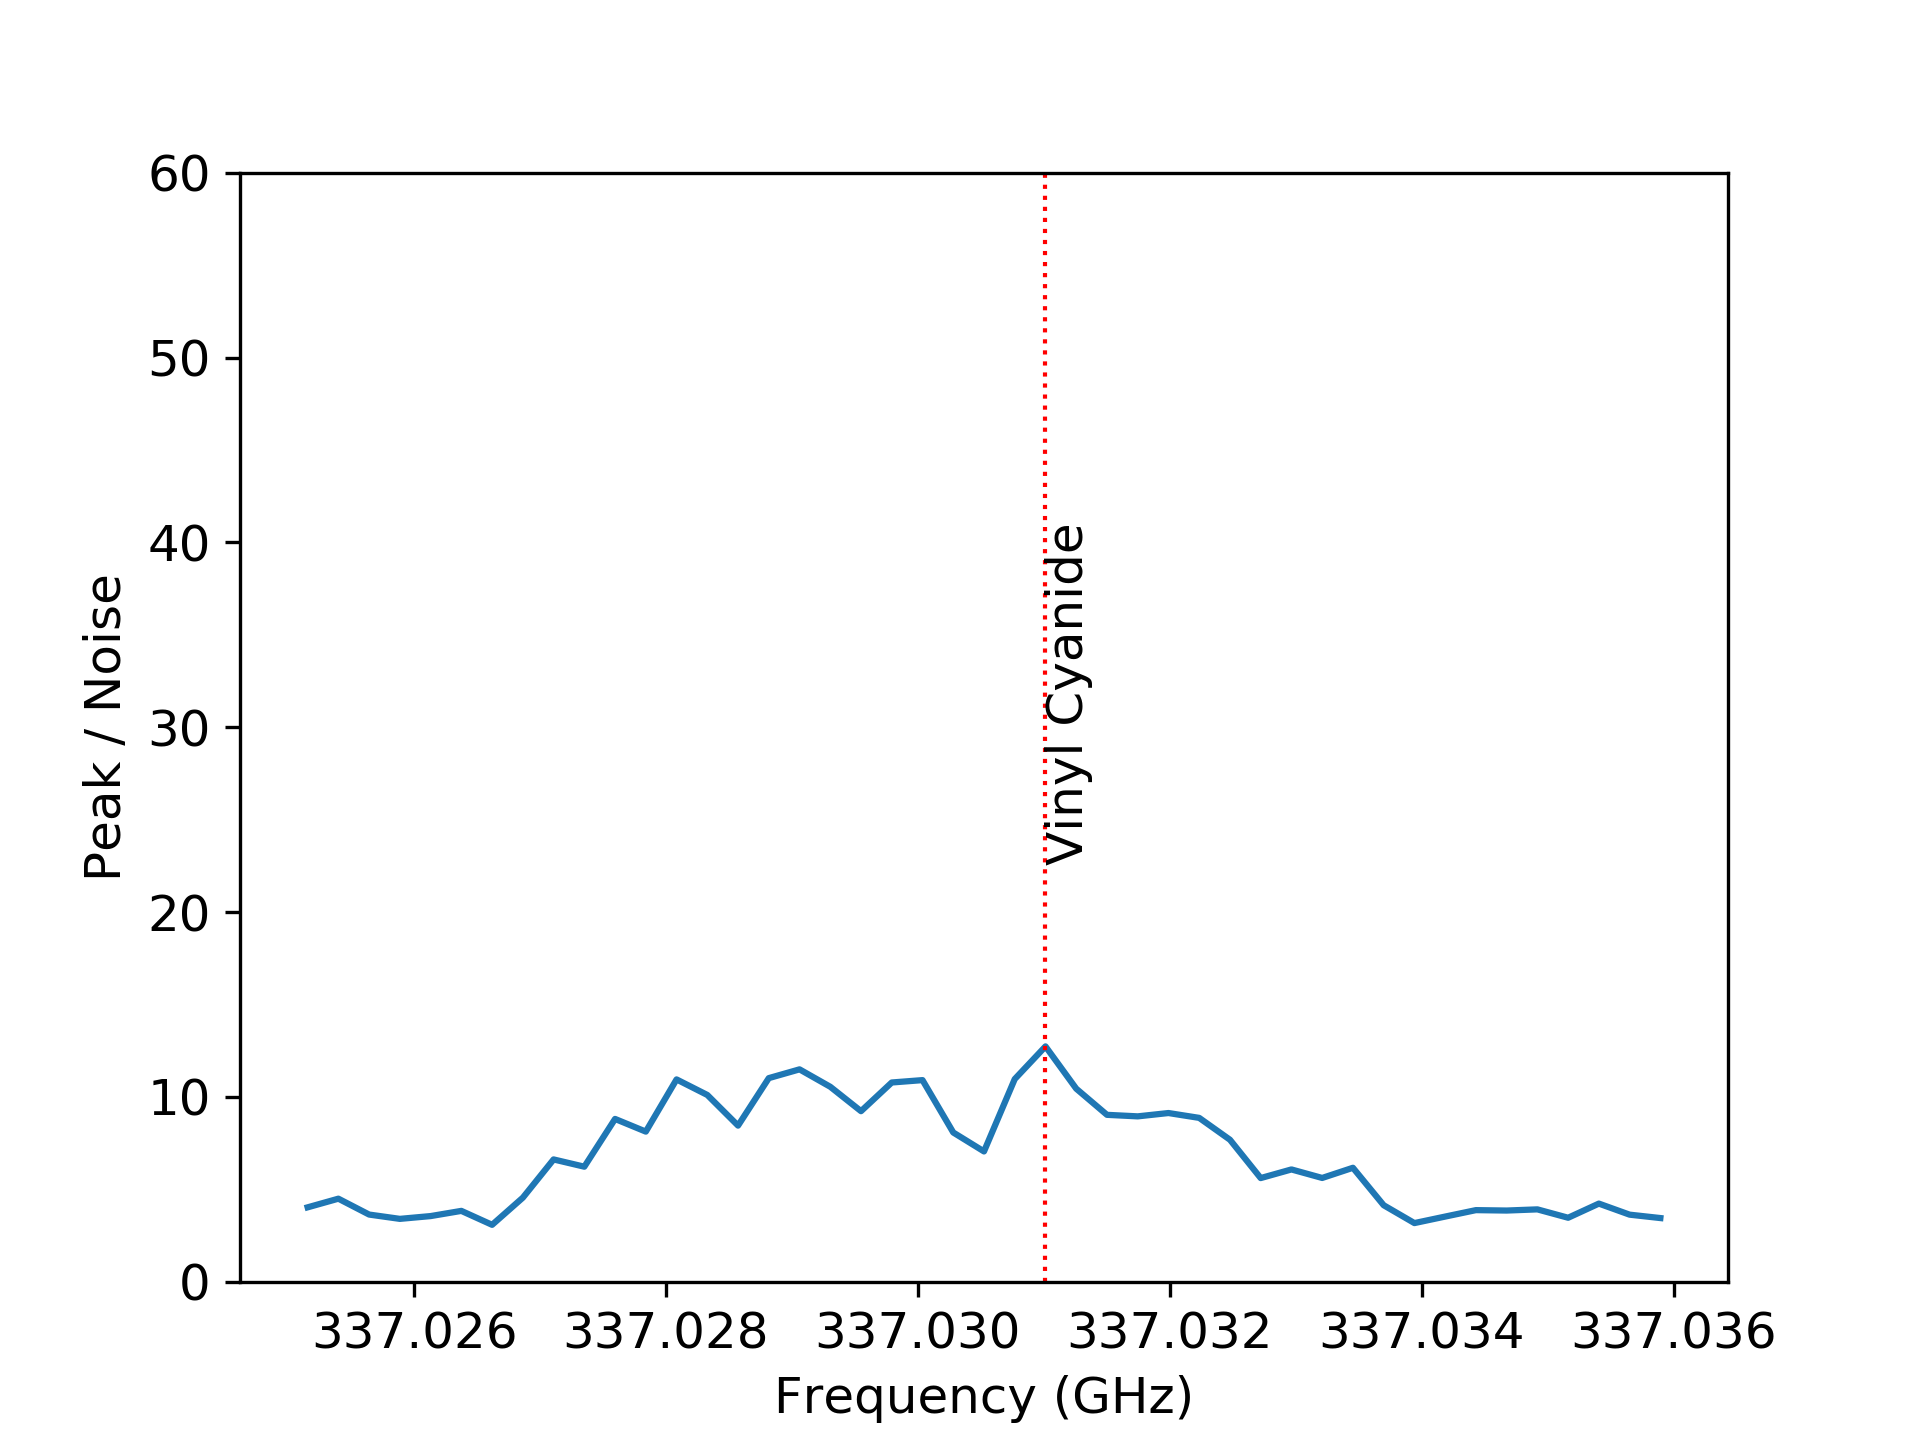
\includegraphics[width=0.33\textwidth]{spw0_CH2CHCN}
    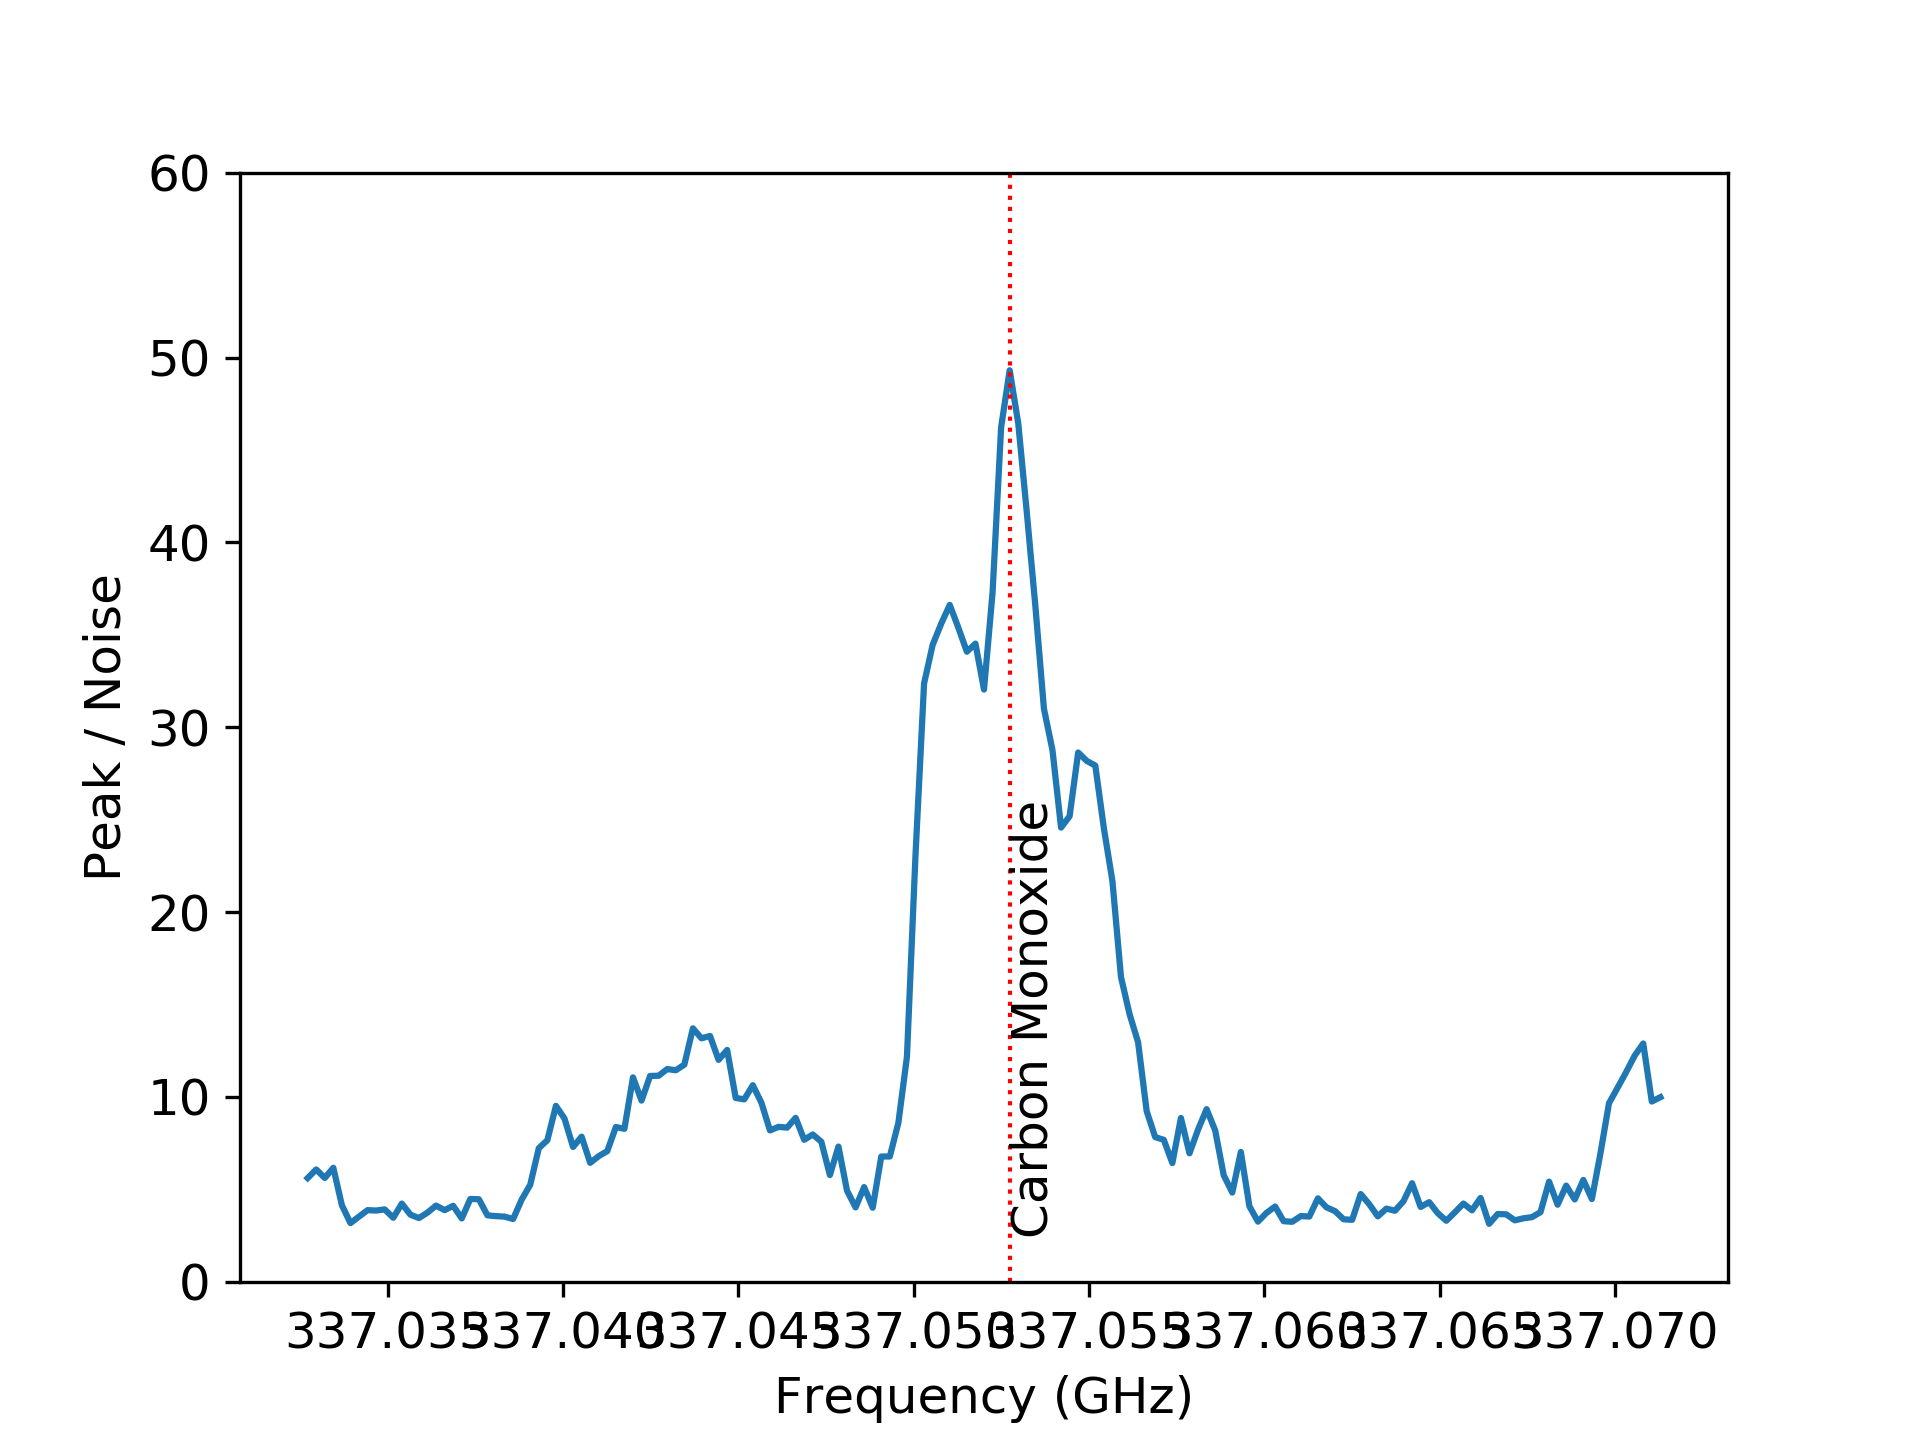
\includegraphics[width=0.33\textwidth]{spw0_C17O}
    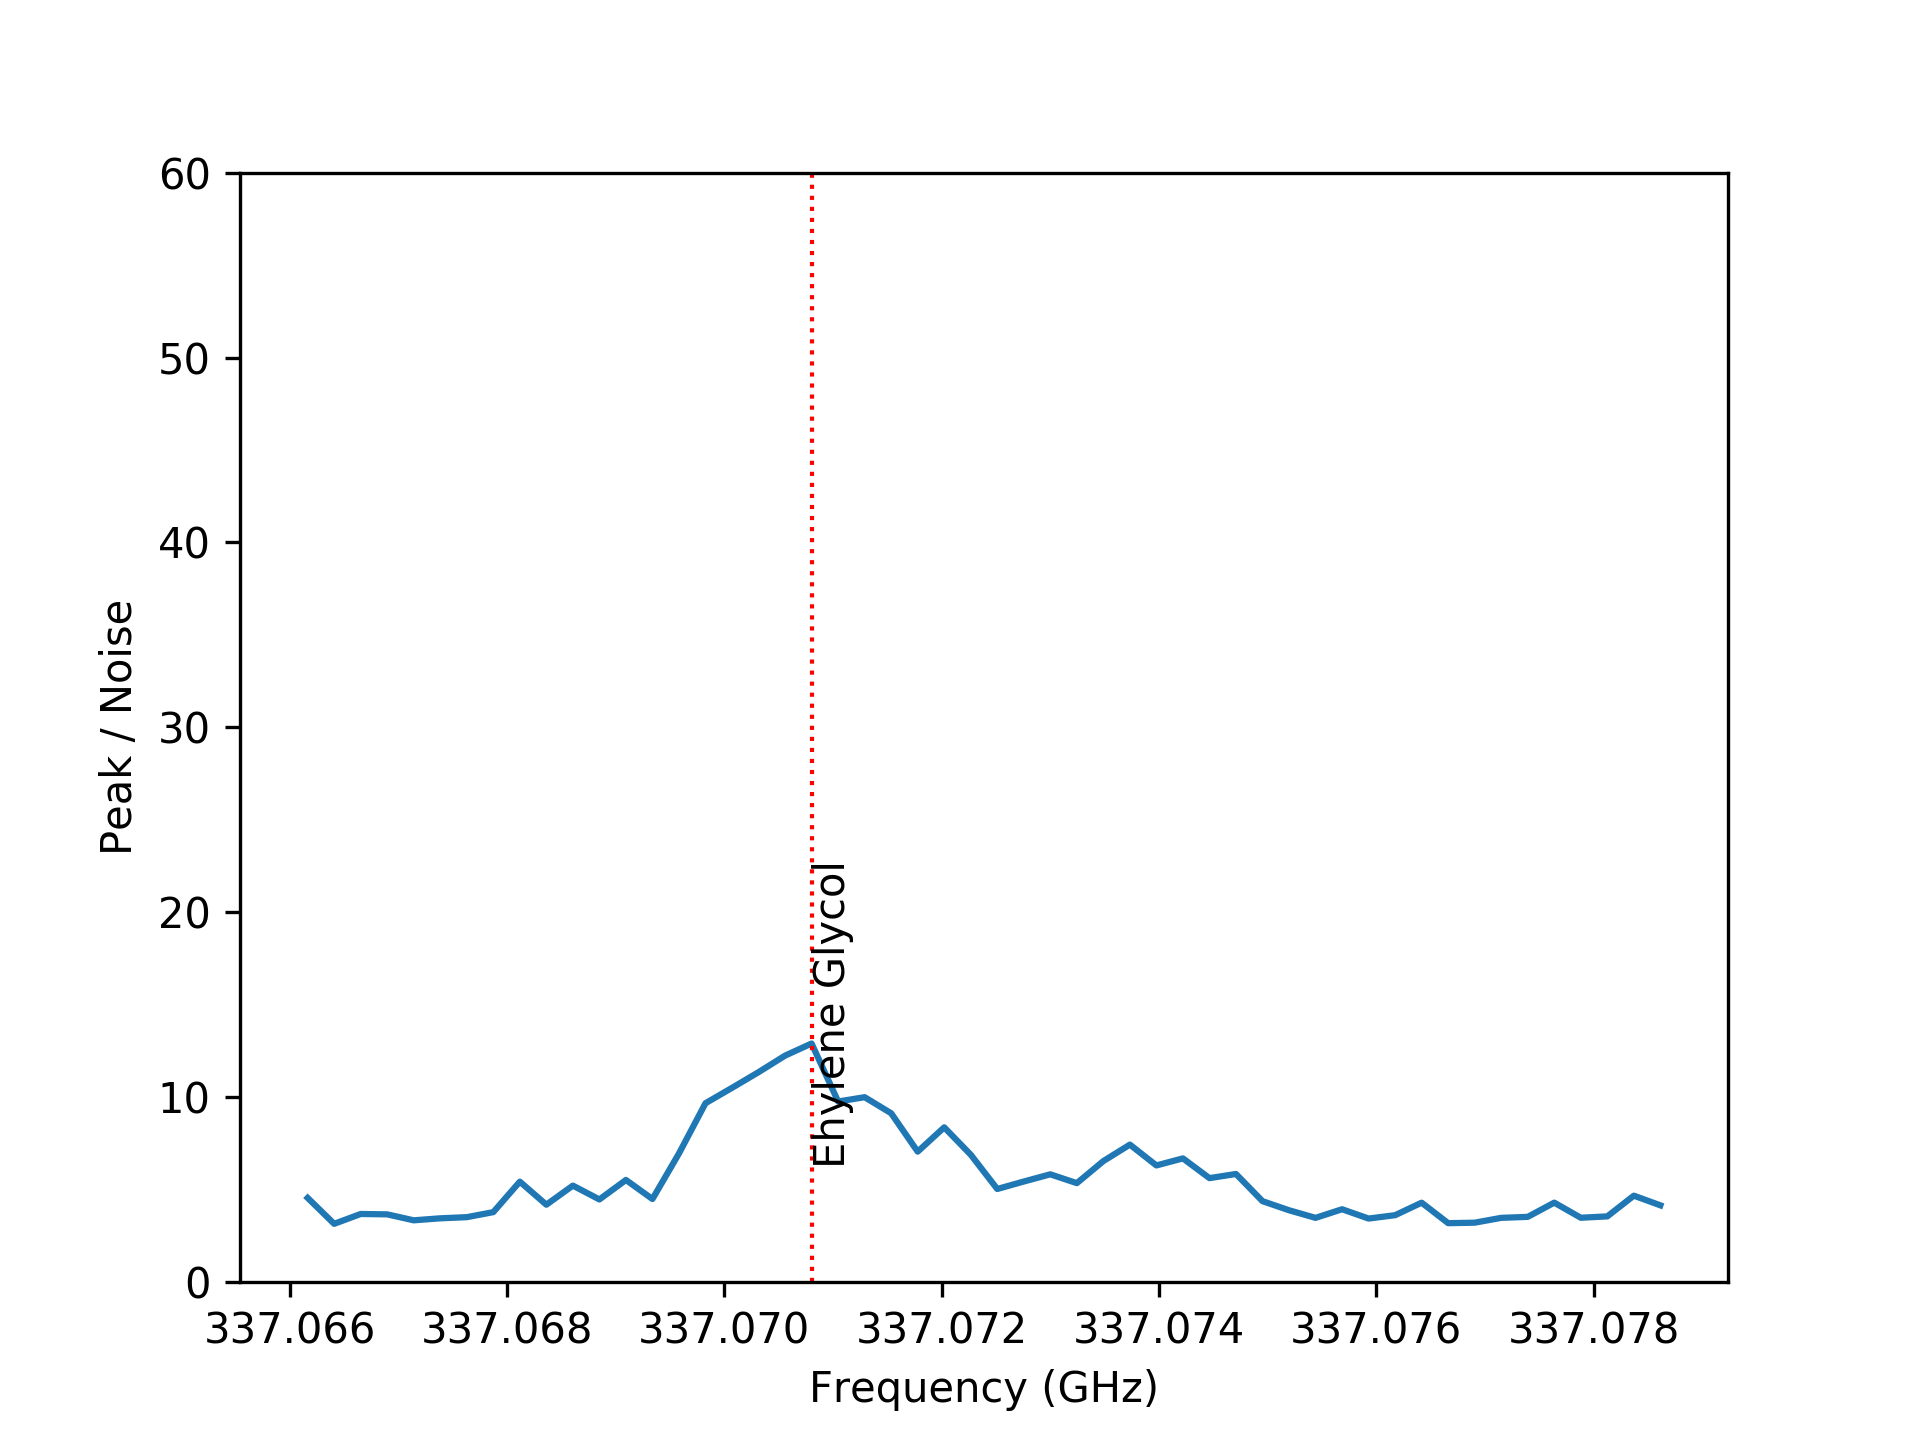
\includegraphics[width=0.33\textwidth]{spw0_(CH2OH)2}
    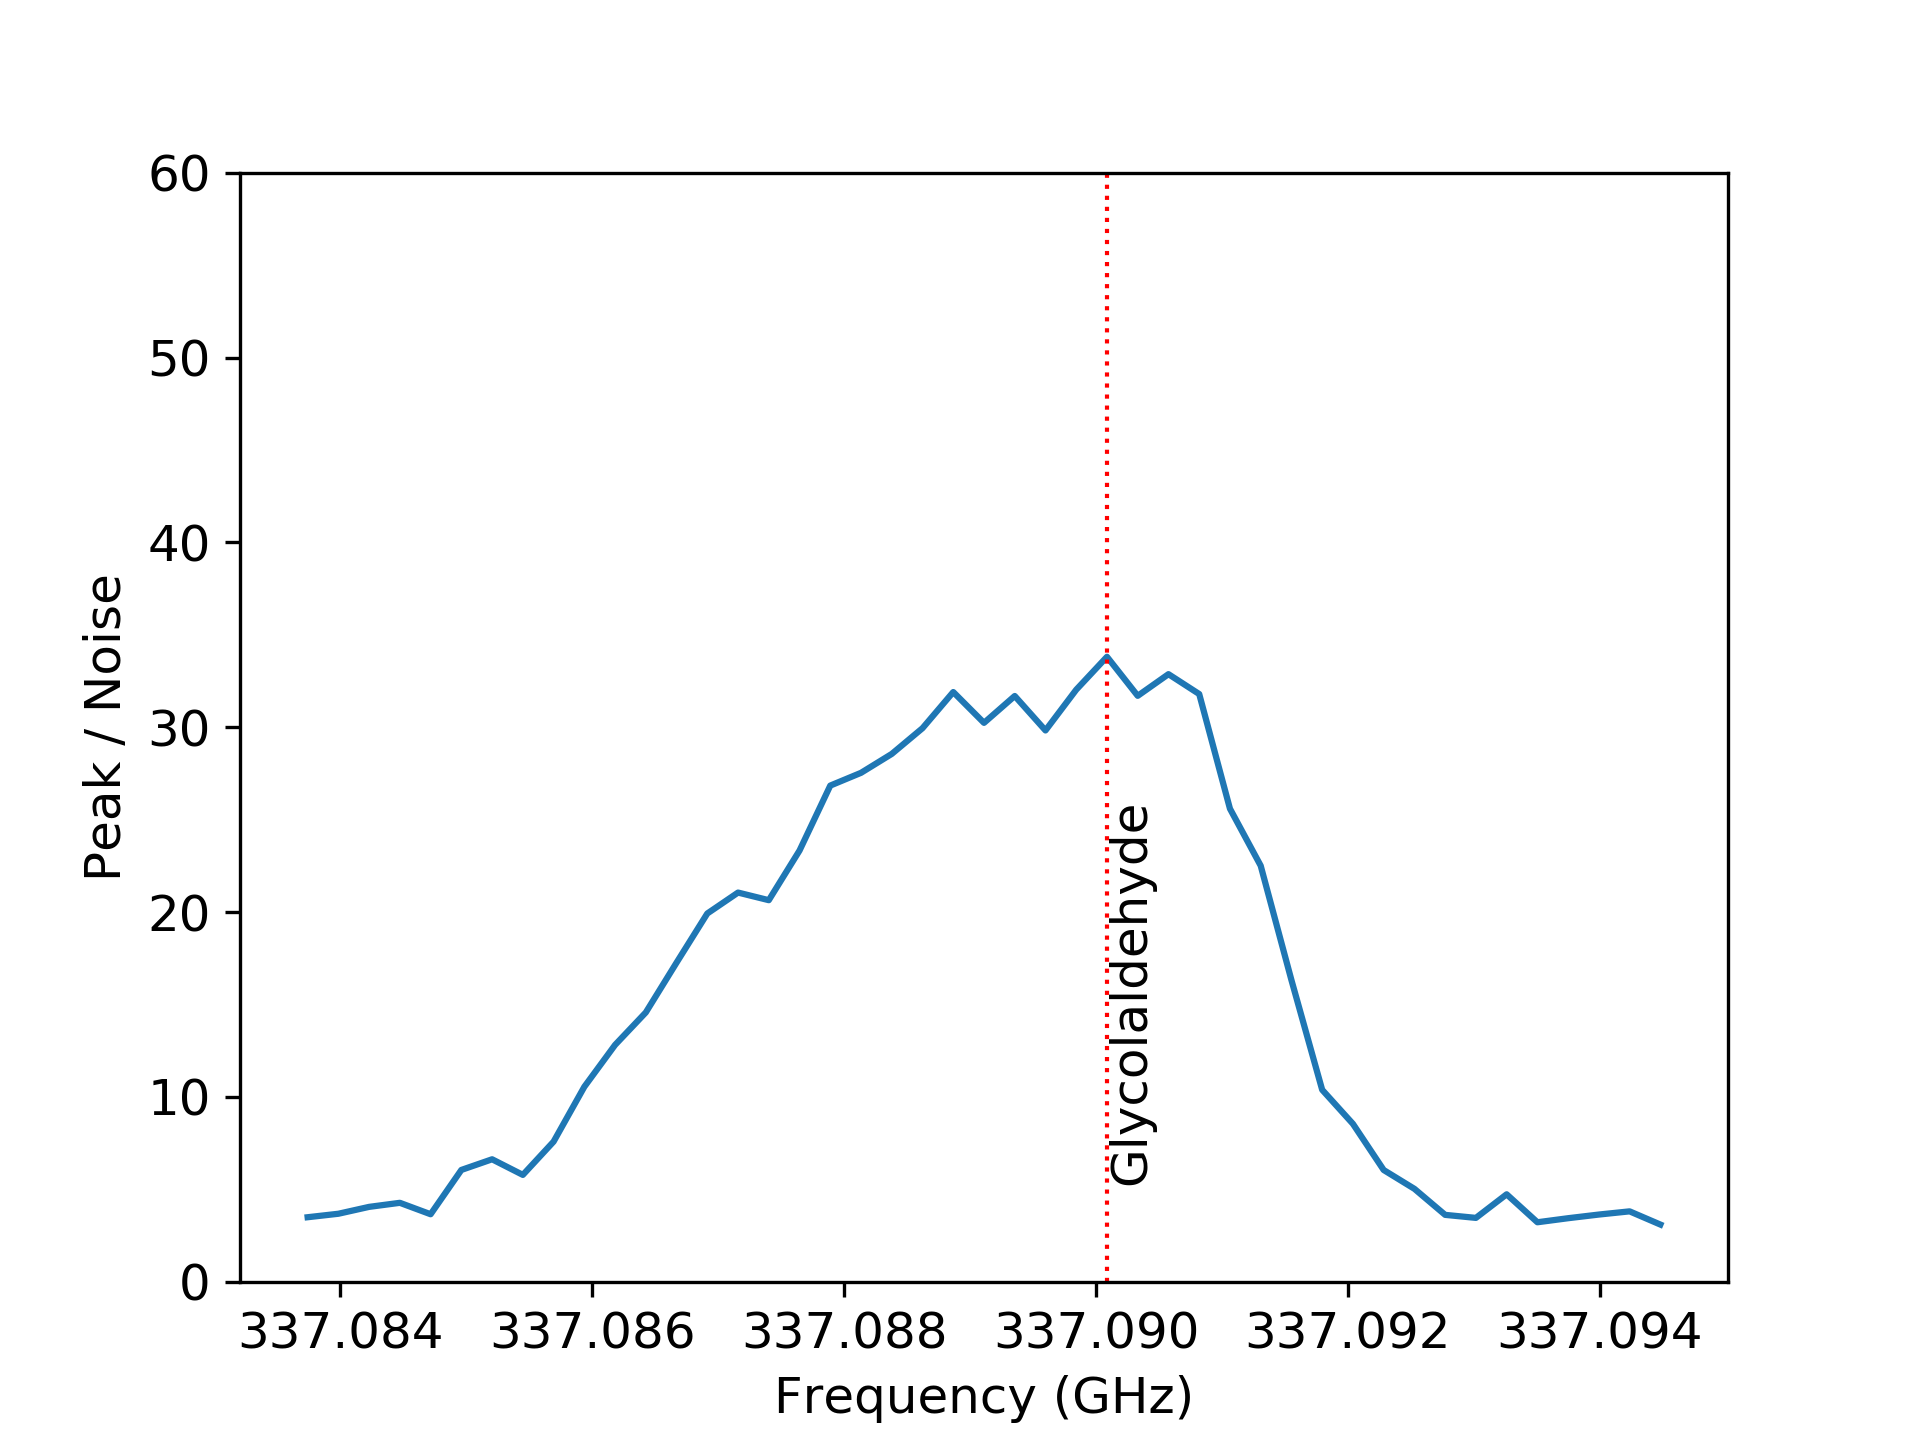
\includegraphics[width=0.33\textwidth]{spw0_CH2OHCHO}
    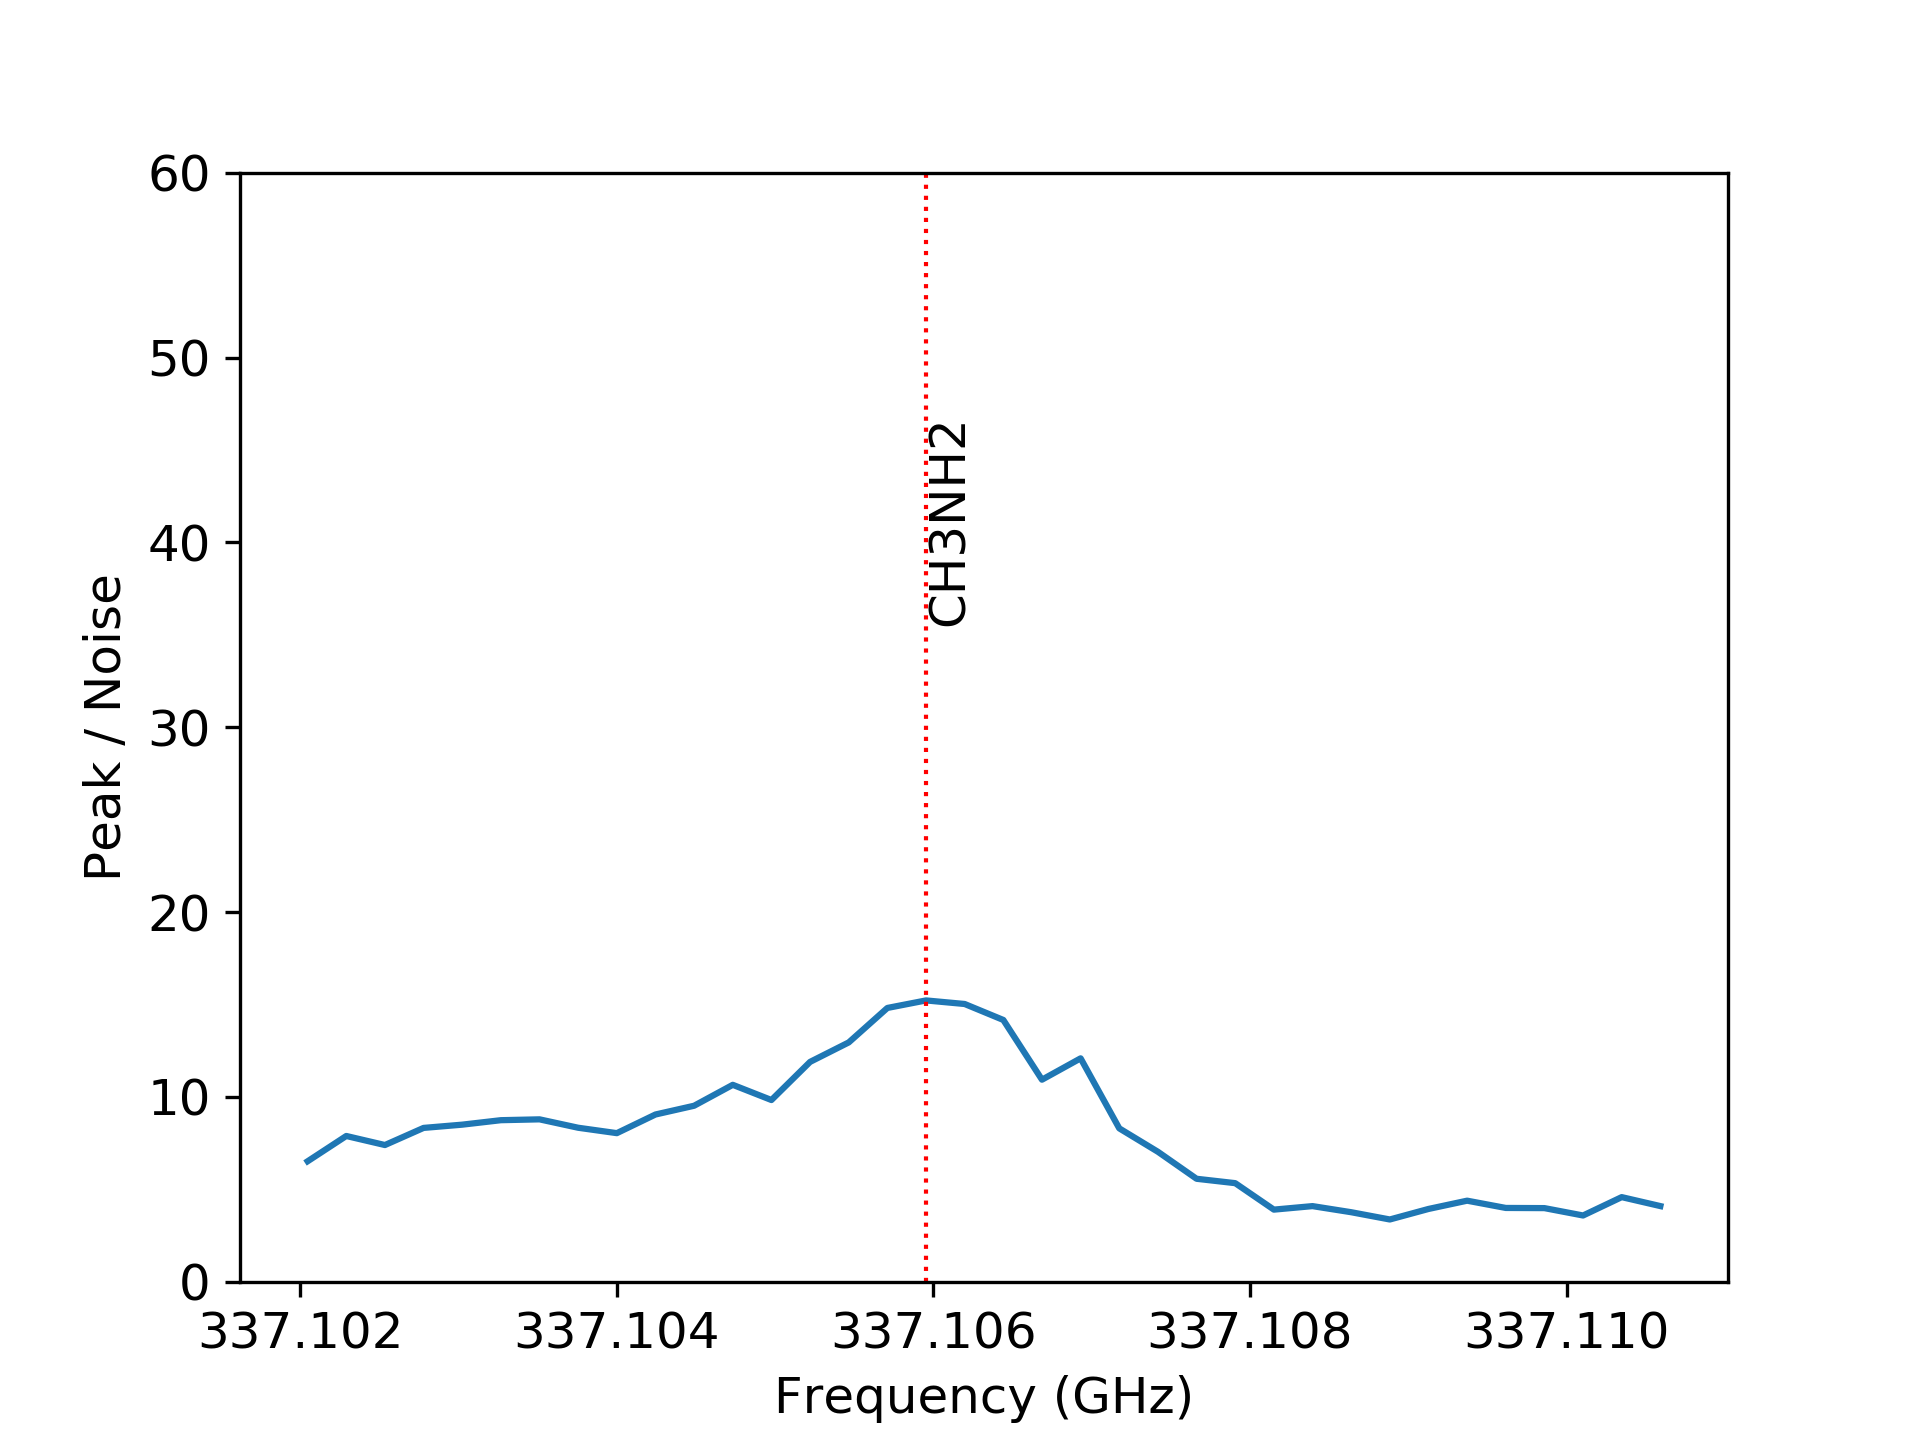
\includegraphics[width=0.33\textwidth]{spw0_CH3NH2}
    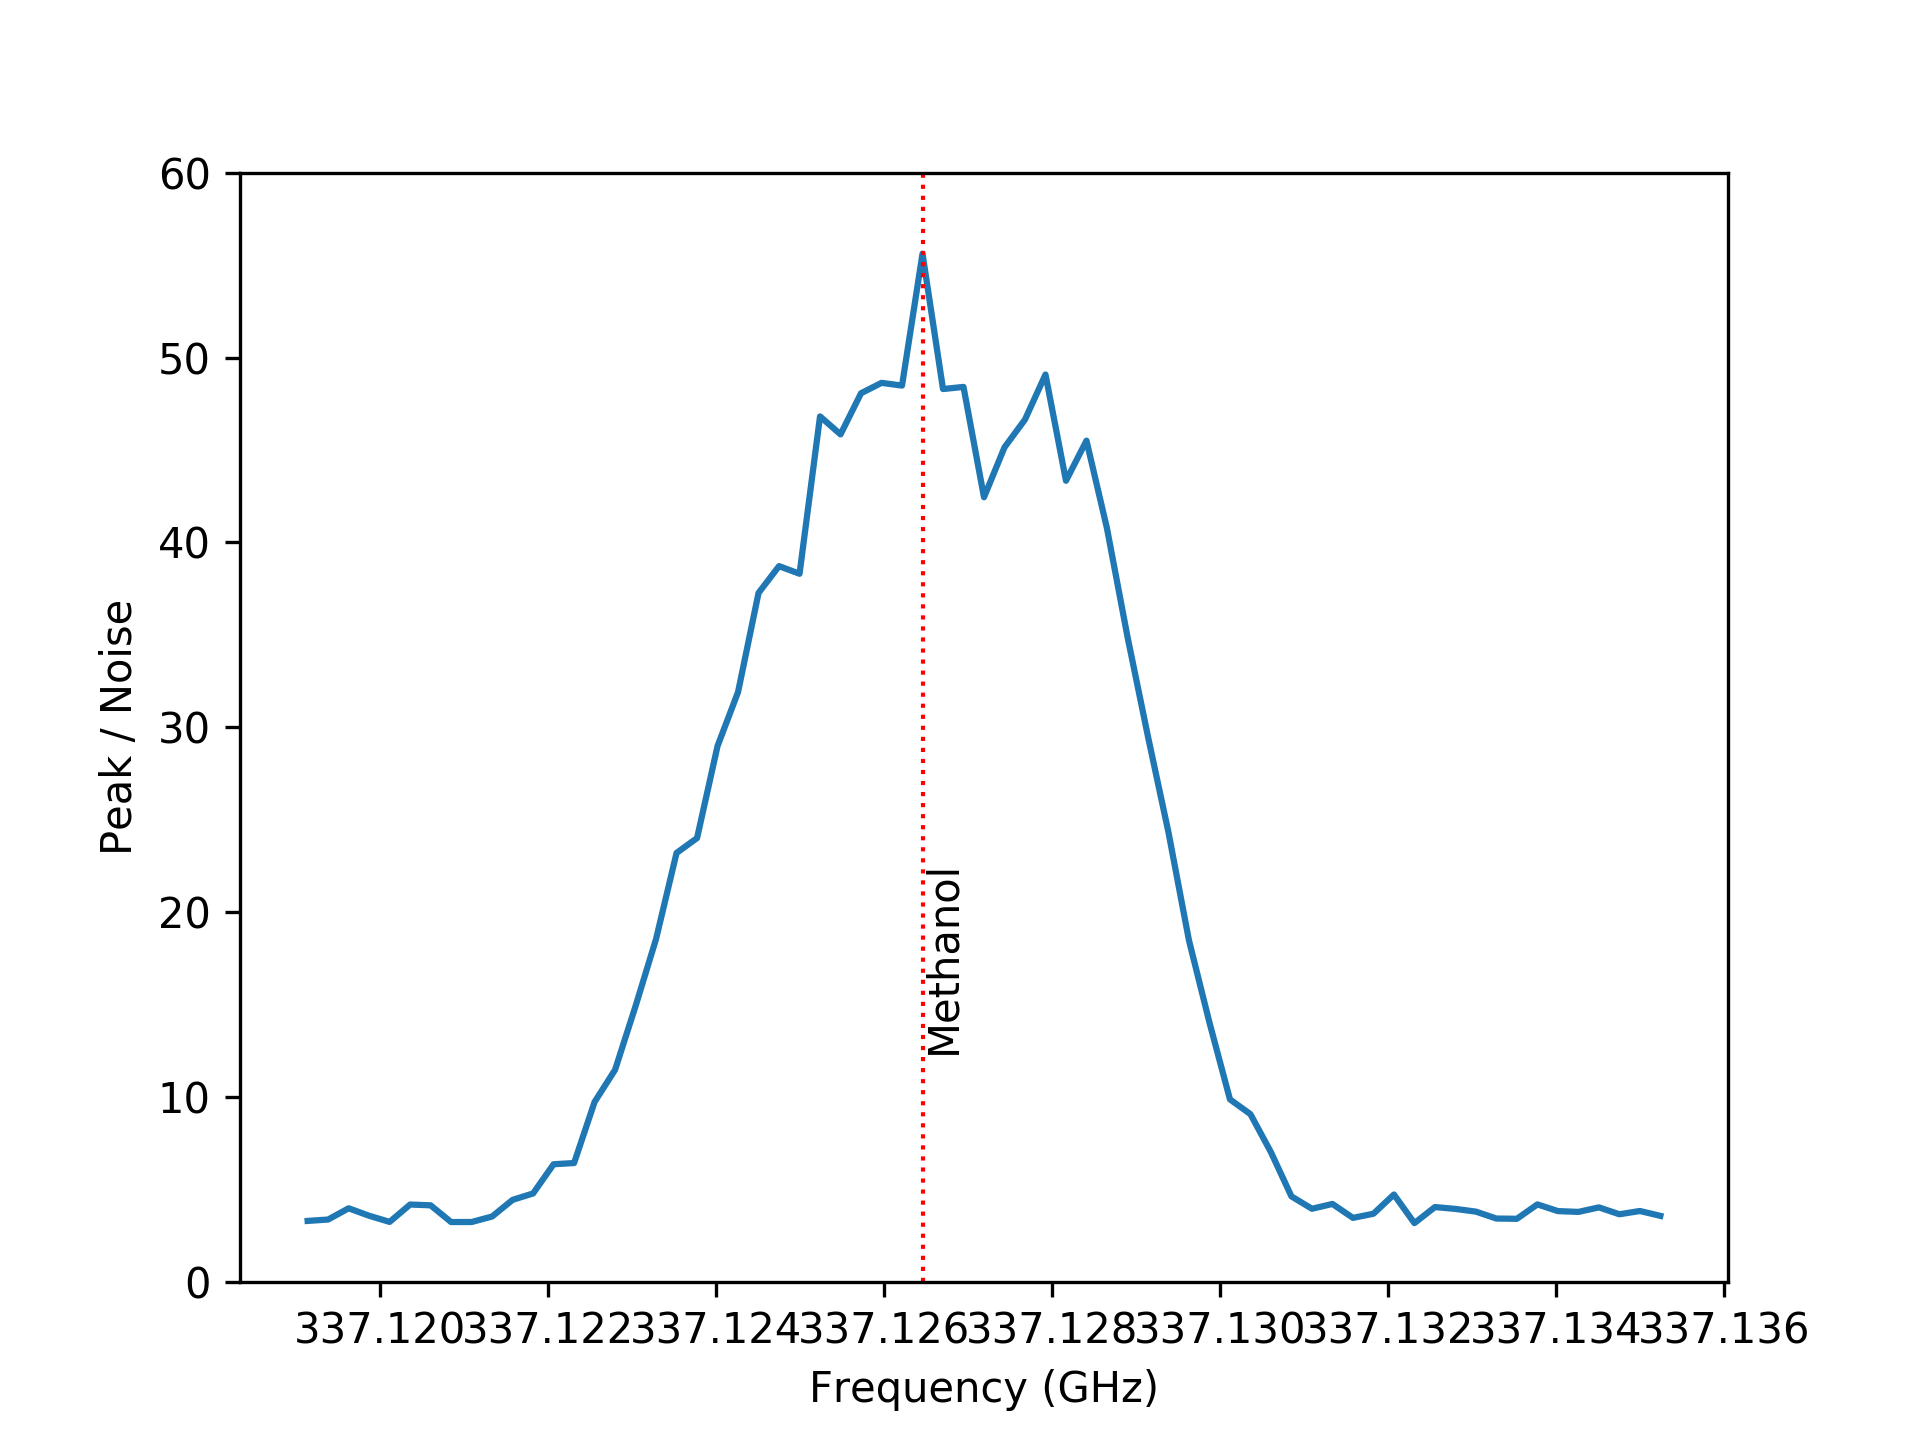
\includegraphics[width=0.33\textwidth]{spw0_CH3OH}
    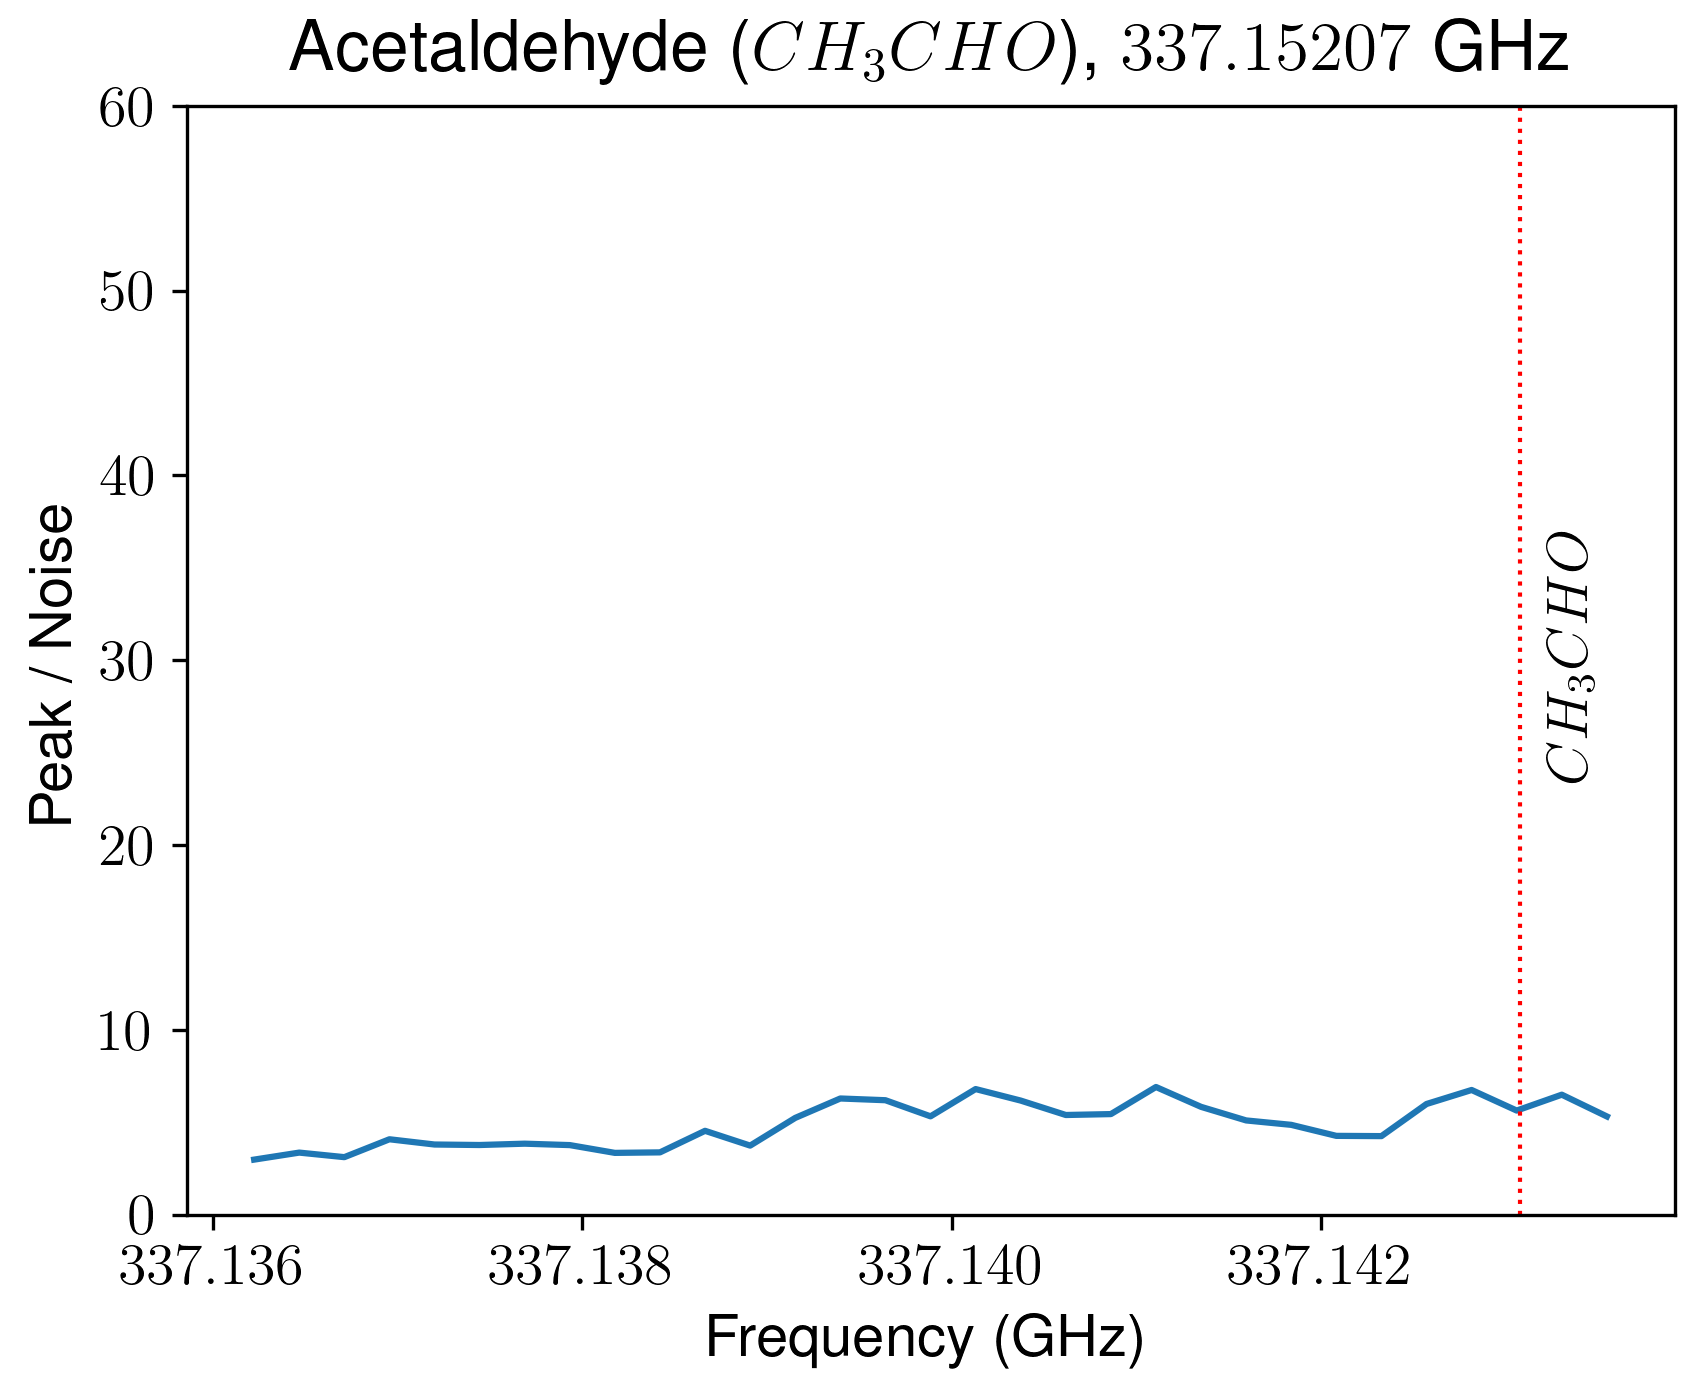
\includegraphics[width=0.33\textwidth]{spw0_CH3CHO}
    
    \caption{Promising molecular lines in spectral window 0}
    
   \end{figure*}



 \begin{table*}   
 \label{table:1}  
     \caption{Line identification results for spectral window 0}
 \tiny
    \centering    
    \begin{tabular}{l l l l l l l l l} 
    \hline\hline       
    Molecule & Name &Transition & Frequency & $E_{u}$ & Intensity & Velocity & $v_{lsr}$ & Peakrms\\ 
    \hline    
$c-HCCCH$ & Cyclopropenylidene & $4_{4,1}-3_{1,2}$ & $336.94859$ & $32.2203$ & $0.4085$ & $7.88862089526$ & $8.0$ & $1.0683$\\
$(CH_{3})_{2}CO$ & Acetone & $33_{1,32}-32_{2,31}EE$ & $336.96839$ & $284.9042$ & $8.7998$ & $8.95064102901$ & $8.0$ & $11.9853$\\
$CH_{2}CH_{13}CN$ & Vinyl Cyanide & $12_{3,10}-11_{2,9}$ & $336.97316$ & $54.8334$ & $2.7746$ & $8.61614536631$ & $8.0$ & $3.779$\\
$(CH_{3})_{2}CO$ & Acetone & $24_{12,13}-23_{11,12}EE$ & $336.97681$ & $230.3935$ & $0.165$ & $7.75784010018$ & $8.0$ & $0.4314$\\
$(CH_{3})_{2}CO$ & Acetone & $45_{28,17}-45_{25,20}AA$ & $336.98001$ & $844.4718$ & $-0.005$ & $8.6029325408$ & $8.0$ & $-1.1173$\\
$(CH_{3})_{2}CO$ & Acetone & $33_{1,32}-32_{2,31}AA$ & $336.98907$ & $284.8304$ & $3.0669$ & $7.56408584877$ & $8.0$ & $4.1771$\\
$_{13}CH_{3}CH_{2}CN$ & Ethyl Cyanide & $55_{1,54}-55_{1,55}$ & $336.99572$ & $634.8624$ & $0.1916$ & $6.78840381265$ & $8.0$ & $0.501$\\
$g'Ga-(CH_{2}OH)_{2}$ & Ethylene Glycol & $69_{18,51}v=1-69_{17,52}v=1$ & $337.00907$ & $1346.1964$ & $0.1628$ & $8.5934862349$ & $8.0$ & $0.4256$\\
$t-H_{13}COOH$ & Formic Acid & $15_{14,2}-14_{14,1}$ & $337.01275$ & $731.763$ & $0.6376$ & $7.05712805295$ & $8.0$ & $0.8684$\\
$H_{2}NCH_{2}CN$ & Aminoacetonitrile & $37_{5,33}-36_{5,32}$ & $337.01833$ & $337.6508$ & $8.4895$ & $8.82510997129$ & $8.0$ & $11.5626$\\
$c-H_{13}CCCH$ & Cyclopropenylidene & $21_{11,10}-21_{11,11}$ & $337.02915$ & $649.5308$ & $0.0$ & $0.0$ & $8.0$ & $0.0$\\
$c-H_{13}CCCH$ & Cyclopropenylidene & $21_{11,10}-21_{10,11}$ & $337.03067$ & $649.5309$ & $8.0889$ & $7.61986732531$ & $8.0$ & $11.017$\\
$CH_{2}CHCN$ & Vinyl Cyanide & $36_{2,35}-35_{2,34}$ & $337.03974$ & $309.7482$ & $6.4719$ & $7.36909982843$ & $8.0$ & $8.8147$\\
$C_{17}O$ & Carbon Monoxide & $J=3-2$ & $337.0611$ & $32.3538$ & $33.3285$ & $0.529522196414$ & $8.0$ & $45.3933$\\
$_{33}SO_{2}$ & Sulfur Dioxide & $5_{5,1}-6_{4,2},F=13/2-15/2$ & $337.07327$ & $75.1261$ & $0.2483$ & $8.49023686004$ & $8.0$ & $0.6492$\\
$g'Ga-(CH_{2}OH)_{2}$ & Ethylene Glycol & $33_{8,25}v=0-32_{8,24}v=1$ & $337.08211$ & $309.0677$ & $6.5759$ & $5.87896210587$ & $8.0$ & $8.9564$\\
$H_{2}CCCHCN$ & Cyanoallene & $67_{1,66}-66_{2,65}$ & $337.08811$ & $560.6032$ & $0.2019$ & $8.10412739257$ & $8.0$ & $0.5279$\\
$(CH_{3})_{2}CO$ & Acetone & $31_{19,13}-31_{16,16}AA$ & $337.09083$ & $401.5121$ & $0.3214$ & $9.26051096965$ & $8.0$ & $0.8403$\\
$cis-CH_{2}OHCHO$ & Glycolaldehyde & $29_{13,17}-28_{13,16}$ & $337.09926$ & $344.463$ & $21.9353$ & $7.5348520422$ & $8.0$ & $29.8758$\\
$cis-CH_{2}OHCHO$ & Glycolaldehyde & $29_{13,16}-28_{13,15}$ & $337.09927$ & $344.463$ & $0.0$ & $0.0$ & $8.0$ & $0.0$\\
$g'Ga-(CH_{2}OH)_{2}$ & Ethylene Glycol & $69_{18,52}v=1-69_{17,53}v=1$ & $337.10336$ & $1346.196$ & $0.2531$ & $7.23270623155$ & $8.0$ & $0.6617$\\
$H_{2}C_{34}S$ & Thioformaldehyde & $10_{7,3}-9_{7,2}$ & $337.10773$ & $732.617$ & $0.2645$ & $7.57139473287$ & $8.0$ & $0.6917$\\
$CH_{3}NH_{2}$ & Methylamine & $2_{2}E2-1-1_{1}E2-1,F=2-2$ & $337.11864$ & $22.2636$ & $0.0$ & $0.0$ & $8.0$ & $0.0$\\
$CH_{3}NH_{2}$ & Methylamine & $2_{2}E2-1-1_{1}E2-1,F=2-1$ & $337.11894$ & $22.2636$ & $8.0177$ & $3.74035836188$ & $8.0$ & $10.9201$\\
$H_{2}C_{34}S$ & Thioformaldehyde & $10_{0,10}-9_{0,9}$ & $337.12546$ & $89.0504$ & $0.2829$ & $8.09050706866$ & $8.0$ & $0.7397$\\
$CH_{3}COOH$ & Acetic Acid & $13_{-6,7}-12_{-4,8}v=0$ & $337.12857$ & $78.4063$ & $0.1969$ & $7.39337397552$ & $8.0$ & $0.5149$\\
$CH_{3}OHvt=_{0}$ & Methanol & $3_{3,0}-4_{2,2}$ & $337.13586$ & $61.6392$ & $37.9398$ & $7.60014640425$ & $8.0$ & $51.6739$\\
$g-CH_{3}CH_{2}OH$ & gauche-Ethanol & $36_{1,36}-35_{2,34},vt=1-0$ & $337.14207$ & $587.8293$ & $0.0009$ & $9.09536620511$ & $8.0$ & $0.1992$\\
$(CH_{3})_{2}CO$ & Acetone & $31_{19,13}-31_{16,16}EA$ & $337.1446$ & $401.4505$ & $-0.1184$ & $7.80215130181$ & $8.0$ & $-0.3097$\\
$CH_{3}CHO$ & Acetaldehyde & $13_{1,12}-12_{-1,12}E$ & $337.15207$ & $88.4514$ & $1.8729$ & $6.9240793504$ & $8.0$ & $2.5509$\\
$g'Ga-(CH_{2}OH)_{2}$ & Ethylene Glycol & $26_{17,9}v=1-26_{16,10}v=1$ & $337.16832$ & $314.6439$ & $0.1946$ & $6.12705989523$ & $8.0$ & $0.5088$\\
$g'Ga-(CH_{2}OH)_{2}$ & Ethylene Glycol & $24_{17,7}v=0-24_{16,8}v=0$ & $337.17585$ & $289.264$ & $0.0$ & $0.0$ & $8.0$ & $0.0$\\


    \hline                  
    \end{tabular}
    
\end{table*}




\section{Conclusions}

   \begin{enumerate}
   \item Item placeholder
   \end{enumerate}


% WARNING
%-------------------------------------------------------------------
% Please note that we have included the references to the file aa.dem in
% order to compile it, but we ask you to:
%
% - use BibTeX with the regular commands:
%   \bibliographystyle{aa} % style aa.bst
%   \bibliography{Yourfile} % your references Yourfile.bib
%
% - join the .bib files when you upload your source files
%-------------------------------------------------------------------

\begin{thebibliography}{}

  \bibitem[Baker(1966)]{baker} Baker, N. 1966,
      in Stellar Evolution,
      ed.\ R. F. Stein,\& A. G. W. Cameron
      (Plenum, New York) 333
\end{thebibliography}

\end{document}
%
%%%%%%%%%%%%%%%%%%%%%%%%%%%%%%%%%%%%%%%%%%%%%%%%%%%%%%%%%%%%%%
Example below of non-structurated natbib references  
To use the v8.3 macros with this form of composition of bibliography, 
the option "bibyear" should be added to the command line 
"\documentclass[bibyear]{aa}".
%%%%%%%%%%%%%%%%%%%%%%%%%%%%%%%%%%%%%%%%%%%%%%%%%%%%%%%%%%%%%%

\begin{thebibliography}{}

  \bibitem[1966]{baker} Baker, N. 1966,
      in Stellar Evolution,
      ed.\ R. F. Stein,\& A. G. W. Cameron
      (Plenum, New York) 333

   \bibitem[1988]{balluch} Balluch, M. 1988,
      A\&A, 200, 58

   \bibitem[1980]{cox} Cox, J. P. 1980,
      Theory of Stellar Pulsation
      (Princeton University Press, Princeton) 16d5

   \bibitem[1969]{cox69} Cox, A. N.,\& Stewart, J. N. 1969,
      Academia Nauk, Scientific Information 15, 1

   \bibitem[1980]{mizuno} Mizuno H. 1980,
      Prog. Theor. Phys., 64, 544
   
   \bibitem[1987]{tscharnuter} Tscharnuter W. M. 1987,
      A\&A, 188, 55
  
   \bibitem[1992]{terlevich} Terlevich, R. 1992, in ASP Conf. Ser. 31, 
      Relationships between Active Galactic Nuclei and Starburst Galaxies, 
      ed. A. V. Filippenko, 13

   \bibitem[1980a]{yorke80a} Yorke, H. W. 1980a,
      A\&A, 86, 286

   \bibitem[1997]{zheng} Zheng, W., Davidsen, A. F., Tytler, D. \& Kriss, G. A.
      1997, preprint
\end{thebibliography}




















%-------------------------------------------------------------
%                 A figure as large as the width of the column
%-------------------------------------------------------------
   \begin{figure}
   \centering
   \includegraphics[width=\hsize]{empty.eps}
      \caption{Vibrational stability equation of state
               $S_{\mathrm{vib}}(\lg e, \lg \rho)$.
               $>0$ means vibrational stability.
              }
         \label{FigVibStab}
   \end{figure}
%
%-------------------------------------------------------------
%                                    One column rotated figure
%-------------------------------------------------------------
   \begin{figure}
   \centering
   \includegraphics[angle=-90,width=3cm]{empty.eps}
      \caption{Vibrational stability equation of state
               $S_{\mathrm{vib}}(\lg e, \lg \rho)$.
               $>0$ means vibrational stability.
              }
         \label{FigVibStab}
   \end{figure}
%
%-------------------------------------------------------------
%                        Figure with caption on the right side 
%-------------------------------------------------------------
   \begin{figure}
   \sidecaption
   \includegraphics[width=3cm]{empty.eps}
      \caption{Vibrational stability equation of state
               $S_{\mathrm{vib}}(\lg e, \lg \rho)$.
               $>0$ means vibrational stability.
              }
         \label{FigVibStab}
   \end{figure}
%
%-------------------------------------------------------------
%                                Figure with a new BoundingBox 
%-------------------------------------------------------------
   \begin{figure}
   \centering
   \includegraphics[bb=10 20 100 300,width=3cm,clip]{empty.eps}
      \caption{Vibrational stability equation of state
               $S_{\mathrm{vib}}(\lg e, \lg \rho)$.
               $>0$ means vibrational stability.
              }
         \label{FigVibStab}
   \end{figure}
%
%-------------------------------------------------------------
%                                      The "resizebox" command 
%-------------------------------------------------------------
   \begin{figure}
   \resizebox{\hsize}{!}
            {\includegraphics[bb=10 20 100 300,clip]{empty.eps}
      \caption{Vibrational stability equation of state
               $S_{\mathrm{vib}}(\lg e, \lg \rho)$.
               $>0$ means vibrational stability.
              }
         \label{FigVibStab}
   \end{figure}
%
%-------------------------------------------------------------
%                                             Two column Figure 
%-------------------------------------------------------------
   \begin{figure*}
   \resizebox{\hsize}{!}
            {\includegraphics[bb=10 20 100 300,clip]{empty.eps}
      \caption{Vibrational stability equation of state
               $S_{\mathrm{vib}}(\lg e, \lg \rho)$.
               $>0$ means vibrational stability.
              }
         \label{FigVibStab}
   \end{figure*}
%
%-------------------------------------------------------------
%                                             Simple A&A Table
%-------------------------------------------------------------
%
\begin{table}
\caption{Nonlinear Model Results}             % title of Table
\label{table:1}      % is used to refer this table in the text
\centering                          % used for centering table
\begin{tabular}{c c c c}        % centered columns (4 columns)
\hline\hline                 % inserts double horizontal lines
HJD & $E$ & Method\#2 & Method\#3 \\    % table heading 
\hline                        % inserts single horizontal line
   1 & 50 & $-837$ & 970 \\      % inserting body of the table
   2 & 47 & 877    & 230 \\
   3 & 31 & 25     & 415 \\
   4 & 35 & 144    & 2356 \\
   5 & 45 & 300    & 556 \\ 
\hline                                   %inserts single line
\end{tabular}
\end{table}

%
%-------------------------------------------------------------
%                                          Table with notes 
%-------------------------------------------------------------
%
% A single note
\begin{table}
\caption{\label{t7}Spectral types and photometry for stars in the
  region.}
\centering
\begin{tabular}{lccc}
\hline\hline
Star&Spectral type&RA(J2000)&Dec(J2000)\\
\hline
69           &B1\,V     &09 15 54.046 & $-$50 00 26.67\\
49           &B0.7\,V   &*09 15 54.570& $-$50 00 03.90\\
LS~1267~(86) &O8\,V     &09 15 52.787&11.07\\
24.6         &7.58      &1.37 &0.20\\
\hline
LS~1262      &B0\,V     &09 15 05.17&11.17\\
MO 2-119     &B0.5\,V   &09 15 33.7 &11.74\\
LS~1269      &O8.5\,V   &09 15 56.60&10.85\\
\hline
\end{tabular}
\tablefoot{The top panel shows likely members of Pismis~11. The second
panel contains likely members of Alicante~5. The bottom panel
displays stars outside the clusters.}
\end{table}
%
% More notes
%
\begin{table}
\caption{\label{t7}Spectral types and photometry for stars in the
  region.}
\centering
\begin{tabular}{lccc}
\hline\hline
Star&Spectral type&RA(J2000)&Dec(J2000)\\
\hline
69           &B1\,V     &09 15 54.046 & $-$50 00 26.67\\
49           &B0.7\,V   &*09 15 54.570& $-$50 00 03.90\\
LS~1267~(86) &O8\,V     &09 15 52.787&11.07\tablefootmark{a}\\
24.6         &7.58\tablefootmark{1}&1.37\tablefootmark{a}   &0.20\tablefootmark{a}\\
\hline
LS~1262      &B0\,V     &09 15 05.17&11.17\tablefootmark{b}\\
MO 2-119     &B0.5\,V   &09 15 33.7 &11.74\tablefootmark{c}\\
LS~1269      &O8.5\,V   &09 15 56.60&10.85\tablefootmark{d}\\
\hline
\end{tabular}
\tablefoot{The top panel shows likely members of Pismis~11. The second
panel contains likely members of Alicante~5. The bottom panel
displays stars outside the clusters.\\
\tablefoottext{a}{Photometry for MF13, LS~1267 and HD~80077 from
Dupont et al.}
\tablefoottext{b}{Photometry for LS~1262, LS~1269 from
Durand et al.}
\tablefoottext{c}{Photometry for MO2-119 from
Mathieu et al.}
}
\end{table}
%
%-------------------------------------------------------------
%                                       Table with references 
%-------------------------------------------------------------
%
\begin{table*}[h]
 \caption[]{\label{nearbylistaa2}List of nearby SNe used in this work.}
\begin{tabular}{lccc}
 \hline \hline
  SN name &
  Epoch &
 Bands &
  References \\
 &
  (with respect to $B$ maximum) &
 &
 \\ \hline
1981B   & 0 & {\it UBV} & 1\\
1986G   &  $-$3, $-$1, 0, 1, 2 & {\it BV}  & 2\\
1989B   & $-$5, $-$1, 0, 3, 5 & {\it UBVRI}  & 3, 4\\
1990N   & 2, 7 & {\it UBVRI}  & 5\\
1991M   & 3 & {\it VRI}  & 6\\
\hline
\noalign{\smallskip}
\multicolumn{4}{c}{ SNe 91bg-like} \\
\noalign{\smallskip}
\hline
1991bg   & 1, 2 & {\it BVRI}  & 7\\
1999by   & $-$5, $-$4, $-$3, 3, 4, 5 & {\it UBVRI}  & 8\\
\hline
\noalign{\smallskip}
\multicolumn{4}{c}{ SNe 91T-like} \\
\noalign{\smallskip}
\hline
1991T   & $-$3, 0 & {\it UBVRI}  &  9, 10\\
2000cx  & $-$3, $-$2, 0, 1, 5 & {\it UBVRI}  & 11\\ %
\hline
\end{tabular}
\tablebib{(1)~\citet{branch83};
(2) \citet{phillips87}; (3) \citet{barbon90}; (4) \citet{wells94};
(5) \citet{mazzali93}; (6) \citet{gomez98}; (7) \citet{kirshner93};
(8) \citet{patat96}; (9) \citet{salvo01}; (10) \citet{branch03};
(11) \citet{jha99}.
}
\end{table}
%-------------------------------------------------------------
%                      A rotated Two column Table in landscape  
%-------------------------------------------------------------
\begin{sidewaystable*}
\caption{Summary for ISOCAM sources with mid-IR excess 
(YSO candidates).}\label{YSOtable}
\centering
\begin{tabular}{crrlcl} 
\hline\hline             
ISO-L1551 & $F_{6.7}$~[mJy] & $\alpha_{6.7-14.3}$ 
& YSO type$^{d}$ & Status & Comments\\
\hline
  \multicolumn{6}{c}{\it New YSO candidates}\\ % To combine 6 columns into a single one
\hline
  1 & 1.56 $\pm$ 0.47 & --    & Class II$^{c}$ & New & Mid\\
  2 & 0.79:           & 0.97: & Class II ?     & New & \\
  3 & 4.95 $\pm$ 0.68 & 3.18  & Class II / III & New & \\
  5 & 1.44 $\pm$ 0.33 & 1.88  & Class II       & New & \\
\hline
  \multicolumn{6}{c}{\it Previously known YSOs} \\
\hline
  61 & 0.89 $\pm$ 0.58 & 1.77 & Class I & \object{HH 30} & Circumstellar disk\\
  96 & 38.34 $\pm$ 0.71 & 37.5& Class II& MHO 5          & Spectral type\\
\hline
\end{tabular}
\end{sidewaystable*}
%-------------------------------------------------------------
%                      A rotated One column Table in landscape  
%-------------------------------------------------------------
\begin{sidewaystable}
\caption{Summary for ISOCAM sources with mid-IR excess 
(YSO candidates).}\label{YSOtable}
\centering
\begin{tabular}{crrlcl} 
\hline\hline             
ISO-L1551 & $F_{6.7}$~[mJy] & $\alpha_{6.7-14.3}$ 
& YSO type$^{d}$ & Status & Comments\\
\hline
  \multicolumn{6}{c}{\it New YSO candidates}\\ % To combine 6 columns into a single one
\hline
  1 & 1.56 $\pm$ 0.47 & --    & Class II$^{c}$ & New & Mid\\
  2 & 0.79:           & 0.97: & Class II ?     & New & \\
  3 & 4.95 $\pm$ 0.68 & 3.18  & Class II / III & New & \\
  5 & 1.44 $\pm$ 0.33 & 1.88  & Class II       & New & \\
\hline
  \multicolumn{6}{c}{\it Previously known YSOs} \\
\hline
  61 & 0.89 $\pm$ 0.58 & 1.77 & Class I & \object{HH 30} & Circumstellar disk\\
  96 & 38.34 $\pm$ 0.71 & 37.5& Class II& MHO 5          & Spectral type\\
\hline
\end{tabular}
\end{sidewaystable}
%
%-------------------------------------------------------------
%                              Table longer than a single page  
%-------------------------------------------------------------
% All long tables will be placed automatically at the end of the document
%
\longtab{
\begin{longtable}{lllrrr}
\caption{\label{kstars} Sample stars with absolute magnitude}\\
\hline\hline
Catalogue& $M_{V}$ & Spectral & Distance & Mode & Count Rate \\
\hline
\endfirsthead
\caption{continued.}\\
\hline\hline
Catalogue& $M_{V}$ & Spectral & Distance & Mode & Count Rate \\
\hline
\endhead
\hline
\endfoot
%%
Gl 33    & 6.37 & K2 V & 7.46 & S & 0.043170\\
Gl 66AB  & 6.26 & K2 V & 8.15 & S & 0.260478\\
Gl 68    & 5.87 & K1 V & 7.47 & P & 0.026610\\
         &      &      &      & H & 0.008686\\
Gl 86 
\footnote{Source not included in the HRI catalog. See Sect.~5.4.2 for details.}
         & 5.92 & K0 V & 10.91& S & 0.058230\\
\end{longtable}
}
%
%-------------------------------------------------------------
%                              Table longer than a single page
%                                            and in landscape, 
%                    in the preamble, use: \usepackage{lscape}
%-------------------------------------------------------------

% All long tables will be placed automatically at the end of the document
%
\longtab{
\begin{landscape}
\begin{longtable}{lllrrr}
\caption{\label{kstars} Sample stars with absolute magnitude}\\
\hline\hline
Catalogue& $M_{V}$ & Spectral & Distance & Mode & Count Rate \\
\hline
\endfirsthead
\caption{continued.}\\
\hline\hline
Catalogue& $M_{V}$ & Spectral & Distance & Mode & Count Rate \\
\hline
\endhead
\hline
\endfoot
%%
Gl 33    & 6.37 & K2 V & 7.46 & S & 0.043170\\
Gl 66AB  & 6.26 & K2 V & 8.15 & S & 0.260478\\
Gl 68    & 5.87 & K1 V & 7.47 & P & 0.026610\\
         &      &      &      & H & 0.008686\\
Gl 86
\footnote{Source not included in the HRI catalog. See Sect.~5.4.2 for details.}
         & 5.92 & K0 V & 10.91& S & 0.058230\\
\end{longtable}
\end{landscape}
}
%
%-------------------------------------------------------------
%               Appendices have to be placed at the end, after
%                                        \end{thebibliography}
%-------------------------------------------------------------
\end{thebibliography}

\begin{appendix} %First appendix
\section{Background galaxy number counts and shear noise-levels}
Because the optical images used in this analysis...
\begin{figure*}%f1
\includegraphics[width=10.9cm]{1787f23.eps}
\caption{Shown in greyscale is a...}
\label{cl12301}
\end{figure*}

In this case....
\begin{figure*}
\centering
\includegraphics[width=16.4cm,clip]{1787f24.ps}
\caption{Plotted above...}
\label{appfig}
\end{figure*}

Because the optical images...

\section{Title of Second appendix.....} %Second appendix
These studies, however, have faced...
\begin{table}
\caption{Complexes characterisation.}\label{starbursts}
\centering
\begin{tabular}{lccc}
\hline \hline
Complex & $F_{60}$ & 8.6 &  No. of  \\
...
\hline
\end{tabular}
\end{table}

The second method produces...
\end{appendix}
%
%
\end{document}

%
%-------------------------------------------------------------
%          For the appendices, table longer than a single page
%-------------------------------------------------------------

% Table will be print automatically at the end of the document, 
% after the whole appendices

\begin{appendix} %First appendix
\section{Background galaxy number counts and shear noise-levels}

% In the appendices do not forget to put the counter of the table 
% as an option

\longtab[1]{
\begin{longtable}{lrcrrrrrrrrl}
\caption{Line data and abundances ...}\\
\hline
\hline
Def & mol & Ion & $\lambda$ & $\chi$ & $\log gf$ & N & e &  rad & $\delta$ & $\delta$ 
red & References \\
\hline
\endfirsthead
\caption{Continued.} \\
\hline
Def & mol & Ion & $\lambda$ & $\chi$ & $\log gf$ & B & C &  rad & $\delta$ & $\delta$ 
red & References \\
\hline
\endhead
\hline
\endfoot
\hline
\endlastfoot
A & CH & 1 &3638 & 0.002 & $-$2.551 &  &  &  & $-$150 & 150 &  Jorgensen et al. (1996) \\                    
\end{longtable}
}% End longtab
\end{appendix}

%-------------------------------------------------------------
%                   For appendices and landscape, large table:
%                    in the preamble, use: \usepackage{lscape}
%-------------------------------------------------------------

\begin{appendix} %First appendix
%
\longtab[1]{
\begin{landscape}
\begin{longtable}{lrcrrrrrrrrl}
...
\end{longtable}
\end{landscape}
}% End longtab
\end{appendix}

%%%% End of aa.dem
